\section{Technical details}


\begin{frame}
  \tableofcontents[currentsection] 
\end{frame}

\begin{frame}
 \heading{Structure of \odeint}
 
 \vspace{2ex}
 \centerline{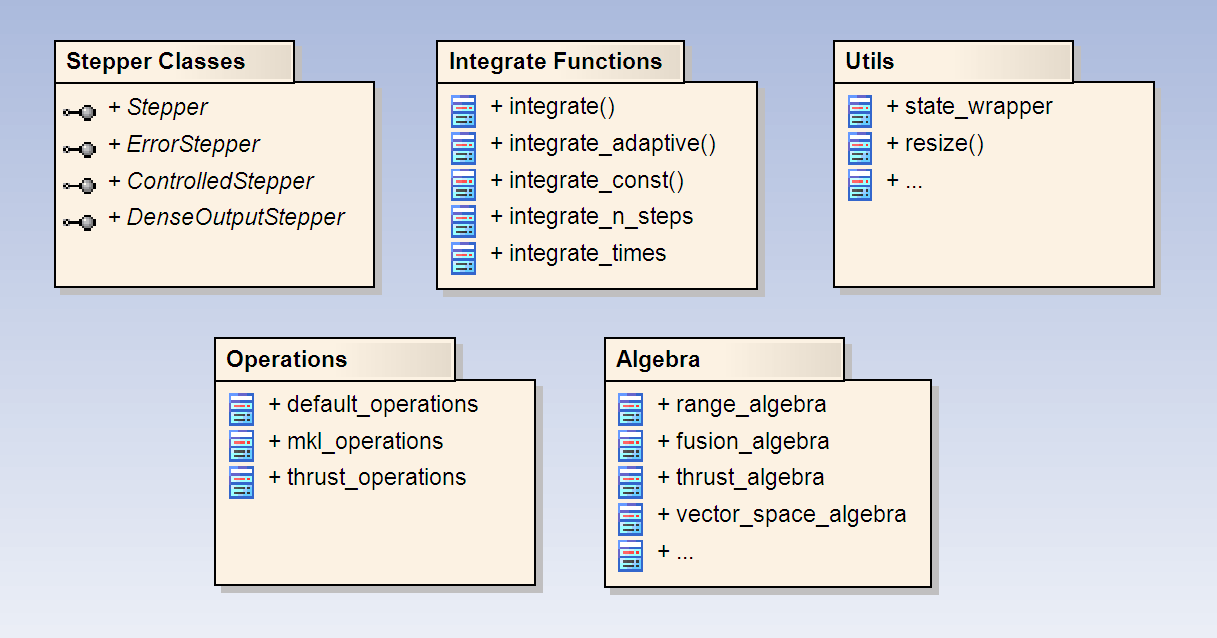
\includegraphics[draft=false,width=1.0\textwidth]{odeint_components.png}}

\end{frame}


\begin{frame}
\heading{Independent Algorithms}
\note{To achive maximum flexibility we wanted to implement the numerical algorithms independent from state type and computation details}

\begin{block}{Goal}
 Container- and computation-independent implementation of the numerical algorithms.  
\end{block}

\begin{block}{Benefit}
 High flexibility and applicability, \odeint\ can be used for virtually any formulation of an ODE.
\end{block}
 
\begin{block}{Approach}
 Detach the algorithm from memory management and computation details and make each part interchangeable.
\end{block}

\end{frame}

\begin{frame}
\heading{Mathematical Algorithm}

 Typical mathematical computation performed to calculate the solution of an ODE ($\dot{\vec x} = \vec f(\vec x , t)$):

\begin{align*}
 \vec F_1 &= \vec f( \vec x_0 , t_0 ) \\
 \vec x' &= \vec x_0 + a_{21} \cdot \Delta t \cdot \vec F_1 \\ \\
 \vec F_2 &= \vec f( \vec x' , t_0 + c_1\cdot\Delta t ) \\
 \vec x' &= \vec x_0 + a_{31} \cdot \Delta t \cdot \vec F_1 + a_{32} \cdot \Delta t \cdot \vec F_2 \\
         &\vdots \\
 \vec x_1 &= \vec x_0 + b_1\cdot \Delta t \cdot \vec F_1 + \dots + b_s\cdot \Delta t \cdot \vec F_s
\end{align*} 

\end{frame}

\begin{frame}[fragile]
\heading{Strucutural Requirements}
\begin{align*}
 {\color{red}\vec F_1} &= \vec f( {\color{red}\vec x_0} , {\color{blue}t_0} ) & %\\
 {\color{red}\vec x'} &= {\color{red}\vec x_0} + {\color{dark-green}a_{21}} \cdot {\color{blue}\Delta t} \cdot {\color{red}\vec F_1}
\end{align*}
 
Types:
\begin{itemize}
 \item {\color{red} vector type}, mostly, but not neccessarily, some container like \texttt{vector<double>} {\scriptsize (actually we have \texttt{state\_type} and \texttt{deriv\_type})}
 \item {\color{blue} time type}, usually \texttt{double}
 \item {\color{dark-green} value type}, fundamental arithmetic type
\end{itemize}
\pause
\vspace{0.5em}

Function Call:
\begin{lstlisting}
void rhs( const vector_type &x , vector_type &dxdt , const time_type t )
{ /* user defined */ }

rhs( x0 , F1 , t ); //memory allocation for F1?
\end{lstlisting}
\begin{itemize}
 \item Memory allocation for temporary results (\lstinline+F1+, \lstinline+x'+)
\end{itemize}

\end{frame}


\begin{frame}
 \heading{Computational Requirements}
\begin{align*}
  \vec x_1 = \vec x_0 + b_1\cdot \Delta t \cdot \vec F_1 + \dots + b_s\cdot \Delta t \cdot \vec F_s
\end{align*}

\begin{itemize}
 \item vector-vector addition
 \item scalar-scalar multiplication
 \item scalar-vector multiplication
\end{itemize}
\vspace{2ex}
\centerline{\small $\longrightarrow$ vector space}

\end{frame}

%\subsection{Memory Management}

\begin{frame}[fragile]
 \heading{Type Declarations}

Tell \odeint\ which types your are working with:

\begin{lstlisting}
/* define your types */
typedef vector<double> state_type;
typedef vector<double> deriv_type;
typedef double value_type;
typedef double time_type;

/* define your stepper algorithm */
typedef runge_kutta4< state_type , value_type , deriv_type , time_type > stepper_type;
\end{lstlisting}

Reasonable standard values for the template parameters allows for:

\begin{lstlisting}
typedef runge_kutta4<state_type> stepper_type;
\end{lstlisting}


\end{frame}



\begin{frame}[fragile]
 \heading{Memory Allocation / Resizing}
Two possible situations: dynamic size / fixed size \lstinline+vector_type+
\vspace{0.5em}

\begin{columns}[t]

 \begin{column}{0.5\linewidth}
  \begin{block}{dynamic size - memory allocation required}
   \begin{itemize}
    \item e.g. \lstinline+vector<double>+
    \item declare type as resizeable
    \item specialize resize template
    \item use \lstinline+initially_resizer+, \lstinline+always_resizer+, or \lstinline+never_resizer+ in stepper
   \end{itemize}
  \end{block}
 \end{column}

 \begin{column}{0.5\linewidth}
  \begin{block}{fixed size - memory allocation not required}
   \begin{itemize}
    \item e.g. \lstinline+array<double,N>+
    \item declare type as not resizeable
    \item that's it
   \end{itemize}
  \end{block}
 \end{column}

\end{columns}

\end{frame}

\begin{frame}[fragile]
 \heading{Declare Resizeability}

\begin{lstlisting}
/* by default any type is not resizable */
template< class Container >
struct is_resizeable
{
    typedef boost::false_type type;
    const static bool value = type::value;
};

/* specialization for std::vector */
template< class T, class A >
struct is_resizeable< std::vector< T , A  > >
{
    typedef boost::true_type type;
    const static bool value = type::value;
}; 
\end{lstlisting}
To use a new dynamic sized type, this has to be specialized by the user.
\end{frame}


\begin{frame}[fragile]
\heading{Tell \odeint\ how to resize}
Again: only required if \\
\centerline{\lstinline+is_resizeable<state_type>::type == boost::true_type+.}
\vspace{0.5em}

Class Template responsible for resizing:
\begin{lstlisting}
template< class StateOut , class StateIn >
struct resize_impl
{
    /* standard implementation */
    static void resize( StateOut &x1 , const StateIn &x2 )
    {
        x1.resize( boost::size( x2 ) );
    }
};
\end{lstlisting}

For anything that does not support \lstinline+boost::size+ and/or \lstinline+resize+ the user must provide a specialization.

\end{frame}


\begin{frame}[fragile]
 \heading{Tell odeint when to resize}
\vspace{2ex}

\begin{lstlisting}
typedef initially_resizer resizer; //default
\end{lstlisting}
Resizing only at first step (memory allocation)

\vspace{1ex}
\begin{lstlisting}
typedef always_resizer resizer;
\end{lstlisting}
Resizing at every step (expanding lattice)

\vspace{1ex}
\begin{lstlisting}
typedef never_resizer resizer;
\end{lstlisting}
Resizing manually by the user (\lstinline+stepper.adjust_size+)

\vspace{2ex}
\begin{lstlisting}
typedef runge_kutta4< state_type , value_type , 
    deriv_type , time_type , algebra , 
    operations , resizer > stepper_type; 
\end{lstlisting}


\end{frame}



\rem{
\begin{frame}[fragile]
 \heading{Scalar Computations}

For the scalar types we require the following:

Assume:
\begin{lstlisting}
time_type t , dt;
value_type a1 , a2 , c;
\end{lstlisting}

Valid Expressions:
\begin{itemize}
 \item \lstinline+a1 = static_cast< value_type >(1)+
 \item \lstinline+a1*a2+, \lstinline+a1/a2+, \lstinline!a1+a2!, \lstinline+a1-a2+, \lstinline+-a1+ 
 \item \lstinline!t + c*dt!
 \item \lstinline!t + dt/c!
 \item \lstinline!t += dt!
\end{itemize}

\end{frame}
}

\begin{frame}[fragile]
 \heading{Vector Computations}

\centerline{$\vec x_1 = \vec x_0 + b_1\cdot \Delta t \cdot \vec F_1 + \dots + b_s\cdot \Delta t \cdot \vec F_s$}

\vspace{0.5em}

Split into two parts:

\begin{description}
 \item[1.~Algebra:] responsible for iteration over vector elements
 \item[2.~Operations:] does the mathematical computation on the elements
\end{description}

\vspace{0.5em}

Similar to \lstinline+std::for_each+

\begin{lstlisting}
Algebra algebra;

algebra.for_each3( x1 , x0 , F1 ,
    Operations::scale_sum2( 1.0, b1*dt );
\end{lstlisting}
\pause

The types \lstinline+Algebra+ and \lstinline+Operations+ are template parameters of the steppers, hence exchangeable.
\end{frame}


\begin{frame}[fragile]
 \heading{Vector Computations}

\begin{lstlisting}
state_type x1, x2, ...
algebra_type algebra;
\end{lstlisting}

Algebra has to have defined the following member functions:

\begin{itemize}
 \item \lstinline+algebra.for_each1( x1 , unary_operation );+
 \item \lstinline+algebra.for_each2( x1, x2, binary_operation );+
 \item \lstinline+algebra.for_each3( ... );+

\[\vdots\]

 \item \lstinline+algebra.for_each15( .. , fifteen_ary_op );+
\end{itemize}

\pause
\odeint\ takes the operations from the class \lstinline+Operations+.

\end{frame}

\begin{frame}[fragile]
 \heading{Operations}

\lstinline+Operations+ is a class with the following member classes:
\begin{itemize}
 \item \lstinline+scale+
 \item \lstinline+scale_sum1+
 \item \lstinline+scale_sum2+
% \item \lstinline+scale_sum3+
\[ \vdots \]
 \item \lstinline+scale_sum14+
\end{itemize}

These classes need a constructor and \lstinline+()+-operator that works together with the algebra:
\begin{lstlisting}
value_type b1, b2;
time_type dt;
algebra.for_each3( x1 , x0 , F1 ,
   Operations::scale_sum2( 1.0, b1*dt );
\end{lstlisting}

This computes: $\vec x_1 = 1.0\cdot \vec x_0 + b_1\Delta t\cdot \vec F_1$.
\end{frame}


\begin{frame}[fragile]
 \heading{Example Implementation: \lstinline+range_algebra+ }

\begin{lstlisting}[basicstyle=\scriptsize\ttfamily]
struct range_algebra {
...
 template< class S1 , class S2 , class S3 , class Op >
 static void for_each3( S1 &s1, S2 &s2, S3 &s3, Op op )
 {
   detail::for_each3( boost::begin(s1), boost::end(s1),
                      boost::begin(s2), boost::begin(s3), 
                      op );
 }
...
};

namespace detail {
...
 template< class Iter1, class Iter2, Iter3, class Op >
 void for_each3( Iter1 first1, Iter1 last1, 
                 Iter2 first2, Iter3 first3, Op op )
 {
     for( ; first1 != last1 ; )
         op( *first1++ , *first2++ , *first3++ );
 }
...
};
\end{lstlisting}

\end{frame}


\begin{frame}[fragile]
 \heading{Example Implementation: \lstinline+default_operations+ }
\begin{lstlisting}
template< class Fac1 , class Fac2 >
struct scale_sum2
{
  const Fac1 m_alpha1;
  const Fac2 m_alpha2;

  scale_sum2( Fac1 alpha1 , Fac2 alpha2 ) 
    : m_alpha1( alpha1 ) , m_alpha2( alpha2 ) 
  { }

  template< class T1 , class T2 , class T3 >
  void operator()( T1 &t1 , const T2 &t2 , const T3 &t3 )
  { t1 = m_alpha1 * t2 + m_alpha2 * t3; }

  typedef void result_type;
};
\end{lstlisting}

\end{frame}

\begin{frame}[fragile]

%\lstinline+range_algebra & default_operations+ can be used with any Container that supports Boost.Range and whose \lstinline+container::value_type+ supports operators \lstinline!+,*!.

For example \lstinline+vector< double >+:
\begin{lstlisting}
typedef vector< double > state_type;
typedef vector< double > deriv_type;
typedef double value_type;
typedef double time_type;

typedef runge_kutta4< state_type , value_type , 
                      deriv_type , time_type , 
                      range_algebra , 
                      default_operations 
                    > stepper_type
\end{lstlisting}

\vspace{1em}
As these are also the default values, this can be shortened:
\begin{lstlisting}
typedef runge_kutta4<state_type> stepper_type; 
\end{lstlisting}

\end{frame}


\begin{frame}[fragile]
 \lstinline+range_algebra & default_operations+ work also with

\begin{itemize}
 \item \lstinline+vector< complex<double> >+
 \item \lstinline+list< double >+
 \item \lstinline+array< double , N >+
\end{itemize}

\pause
What about
\begin{itemize}
 \item Ublas \lstinline+vector+
 \item trivial \lstinline+state_type+ like \lstinline+double+
 \item generally: \lstinline+state_type+ that support operators \lstinline!+,*!
\end{itemize}

\vspace{1em}
\centerline{$\longrightarrow$ \lstinline+vector_space_algebra+!}

\end{frame}


\begin{frame}[fragile]
 \heading{\lstinline+vector_space_algebra+}

\begin{lstlisting}
struct vector_space_algebra {
...
 template< class S1 , class S2 , class S3 , class Op >
 static void for_each3( S1 &s1 , S2 &s2 , 
                        S3 &s3 , Op op )
 {
   op( s1 , s2 , s3 );
 }
...
};
\end{lstlisting}

\begin{itemize}
 \item delegates \lstinline+state_type+ directly to the operations 
 \item no iteration
 \item works together with \lstinline+default_operations+ with any \lstinline+state_type+ that supports operators \lstinline!+,*!
\end{itemize}

\end{frame}


\begin{frame}[fragile]
 \heading{Other Examples}

\begin{description}
 \item[fusion\_algebra:] works with compile-time sequences like \lstinline+fusion::vector+ of Boost.Units
 \item[thrust\_algebra \& thrust\_operations:] Use thrust library to perform computation on CUDA graphic cards
 \item[mkl\_operations:] Use Intel's Math Kernel Library
 %\item[nested\_algebra:] can handle nested containers that support Boost.Range, e.g.\ \lstinline+vector< vector<double> >+
\end{description}

See tutorial and documentation on \verb+www.odeint.com+ for more.

\pause
\vspace{0.5em}
\begin{block}{Important}
 Division into Algebra and Operations gives us great flexibility. However, state type, algebra and operations must coorporate to make \odeint\ work!
\end{block}

\end{frame}

\begin{frame}
 \heading{More details}

\vspace{2ex}
\begin{itemize}
 \item State wrapper for construction/destruction of state types
 \item More requirements on Algebras when using controlled steppers (\lstinline+algebra.reduce+)
 \item Implicit routines using Ublas
 \item Generation functions to create controlled / dense output steppers
 \item TMP Runge-Kutta implementation (see my talk on Thursday afternoon!)
\end{itemize}

\end{frame}

